\section{Antenner -- allmänt}
\index{antenner}

Aldrig så förnämliga radioapparater kommer inte till sin fulla rätt
utan ett effektivt antennsystem. Det är en huvudförutsättning för
framgångsrik radiokommunikation.

Antennen omsätter elektrisk energi från sändaren till
elektromagnetiska fält som strålas ut, d.v.s. radiovågor.

Vid mottagning fångar antennen upp radiovågorna och omsätter dem till
elektriska signaler som förs till mottagaren.

Antennsystemet består av den egentliga antennen och
transmissionsledningen mellan denna och sändaren respektive
mottagaren. I antennsystemet ingår även impedansanpassningar,
antennkopplare m.m.


\subsubsection{Våghastighet}
\label{ljushastigheten}
\index{våghastighet}
\index{ljushastighet}
\index{dielektricitetskonstant}
\index{permabilitetetskonstant}
\index{frekvens}

I vakuum breder elektromagnetiska vågor ut sig med hastigheten
\(c_0\), vilken mest kallas ljushastigheten.

\[c_0 \approx 300 \cdot 10^6 \text{ [m/s]}\]

I andra media än vakuum har samma vågor utbredningshastigheten
\(c\). Formeln är då

\[c = \frac{c_0}{\sqrt{µ_o \cdot \varepsilon_r}}\]

där \(µ_0\) är relativa permeabilitetskonstanten och \(\varepsilon_0\)
är relativa dielektricitetskonstanten för det medium som vågorna
passerar igenom.  För enkelhetens skull sätts här \(µ_0\) och
\(\varepsilon_0\) till 1, alltså \(c_0 = c\).

Sambandet mellan våghastigheten i vakuum, frekvensen och våglängden är förenklat

\[ c = \lambda \cdot f \quad c\text{ [m/s] }\quad f\text{ [Hz] } \quad \lambda\text{ [m]}\]

och våglängden således

\[ \lambda = \frac{c}{f} \quad \text{[m]} \]

\subsection{Antennlängd}

\subsubsection{Elektriska längden}
\index{elektrisk längd}
\index{antenn!elektrisk längd}

Längden för en resonant, ideal antenn som är en våglängd lång kan
beräknas med ovanstående formel. Vi kallar denna längd för den
\emph{elektriska} längden. Således \(l_e = \lambda\).

Elektriska längden (\(l_e\)) för en halvvågsantenn (\(\lambda/2\))
är hälften av den elektriska längden för en helvågsantenn
(\(\lambda\)):

\[l_e = \frac{c}{2f} \quad \text{[m]}\]

\subsubsection{Mekaniska längden}
\index{mekanisk längd}
\index{antenn!mekanisk längd}
\index{förkortningsfaktor}
\index{antenn!förkortningsfaktor}
\index{resonansfrekvens}
\index{antenn!resonansfrekvens}

Man skiljer på antennens elektriska och mekaniska längd. Av flera
orsaker blir den mekaniska antennlängden (\(l_m\)) för samma
frekvens kortare än den elektriska (\(l_e\)). Det beror bl.a. på
våghastighet och ledningsförmåga i de material som ingår samt övriga
elektriska egenskaper beroende på antennens mekaniska utförande,
påverkan från jordplan och omgivning m.m.

Ett förhållande mellan längd och tjocklek av 10000 ger t.ex. en ca 2~\%
mekaniskt kortare antenn.
Förhållandet 30 ger en ca 5~\% kortare antenn.
Det första värdet kan passa för en 2~mm tjock halvvågsantenn för 7~MHz.
Det andra värdet för en 3,5~mm tjock halvvågsantenn för 145~MHz.
Diagram för den s.k. förkortningsfaktorn finns i de flesta antennhandböcker.

I följande formel har den mekaniska längden (\(l_m\)) för en fritt upphängd
trådantenn valts 2~\% kortare än den elektriska längden.

\[l_m = \frac{c}{2f} \cdot 0,98 = \frac{147\cdot 10^6}{f} \quad \text{[m]}\]

Exempel: Beräkna den elektriska och mekaniska längden på en halvvågsantenn med
resonansfrekvensen \(f = 7\) MHz.

\[
c = \lambda \cdot f
\quad c\ \text{[m/s]} \quad f\ \text{[Hz]} \quad \lambda \text{[m]}
\]

Elektriska våglängden för 7~MHz är

\[
\lambda = \frac{c}{f} = \frac{300 \cdot 10^6}{7 \cdot 10^6} = 42,86
\quad \text{[m]}
\]

Antennen är en halvvågsantenn, således är elektriska längden

\[
l_e = \frac{\lambda}{2} = \frac{42.86}{2} = 21,43 \quad \text{[m]}
\]

och mekaniska längden

\[
l_m = \frac{\lambda}{2f} \cdot 0,98 = \frac{42.86}{2}\cdot 0,98 = 21
\quad \text{[m]}
\]


\subsection{Ström och spänning i en halvvågsantenn}
\textbf{
HAREC a.\ref{HAREC.a.6.2.1}\label{myHAREC.a.6.2.1}
}
\index{halvvågsantenn}
\index{antenn!halvvåg}
\index{antenn!ström och spänning}

\begin{wrapfigure}{R}{0.5\textwidth}
  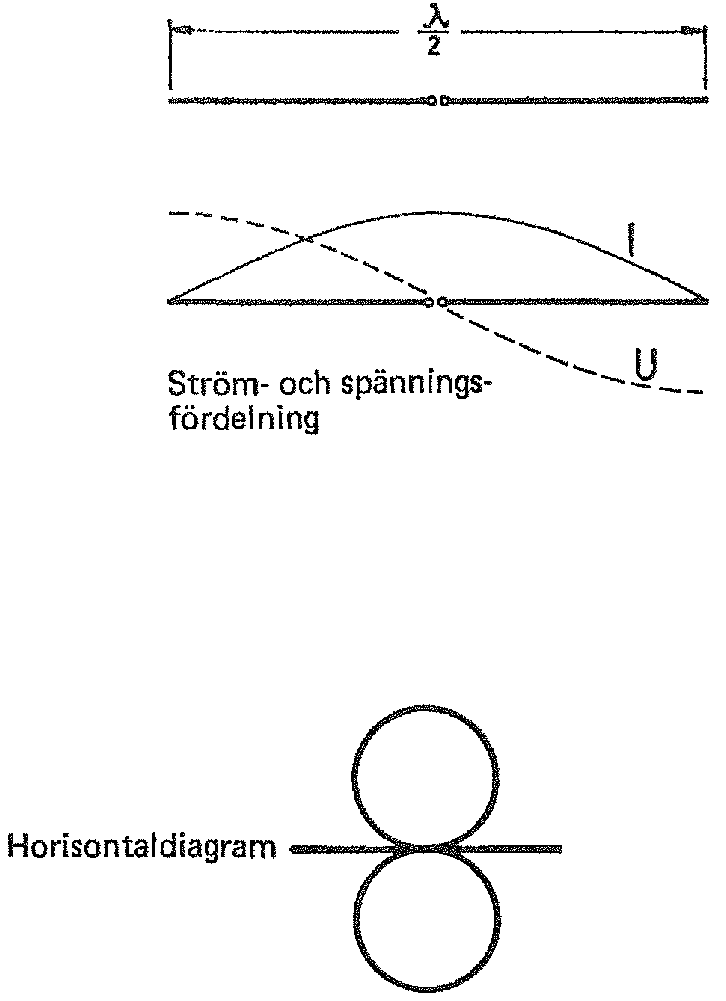
\includegraphics[width=0.5\textwidth]{images/bild_2_6-01.png}
  \caption{Spänning och ström i en halvvågsantenn}
  \label{fig:bildII6-1}
\end{wrapfigure}

När en halvvågsantenn matas med HF-energi på grundfrekvensen, så
uppstår en stående våg med ett typiskt utseende.

Bild \ref{fig:bildII6-1} visar att i vardera änden av antennen uppnår spänningen
\(U\) ett maximum (en spänningsbuk), i mitten uppnår strömmen \(I\)
ett maximum (en strömbuk).  Antennen strålar mest där strömbuken
finns.

Tag t.ex. en 40~meter lång metalltråd som antenn. Dess
grundresonansfrekvens är ca 3,5~MHz, men den är även i resonans på de
harmoniska övertonerna (7, 14, 21, 28~MHz o.s.v.).

Bild \ref{fig:bildII6-3} visar ström- och spänningsfördelningen på antennen vid de
respektive övertonerna.

80~m (3,5~MHz): I matningpunkten står ett spänningsminimum (en
spänningsnod) och ett strömmaximum (en strömbuk). Strömmen är hög
därför att matningspunkten har låg impedans.

Samma antenn på 40~m, 20~m, 15~m, 10~m (7, 14, 21, 28~MHz) har ett
spänningsmaximum (spänningsbuk) och ett strömminimum (strömnod) i
matningspunkten, som då har hög impedans.

Ur horisontaldiagrammet för antennen kan utläsas att ytterligare
strålningskäglor (strålningslober) utvecklas för varje överton i den
påmatade frekvensen. Samtidigt blir strålningen alltmer till riktad
längs med antennen.

\subsection{Impedansen i antennens matningspunkt}
\textbf{
HAREC a.\ref{HAREC.a.6.2.2}\label{myHAREC.a.6.2.2}
}
\index{impedans!antenn}
\index{antenn!impedans}
\index{halvvågsantenn}
\index{antenn!halvvågs}
\index{överton}

\begin{wrapfigure}{R}{0.5\textwidth}
  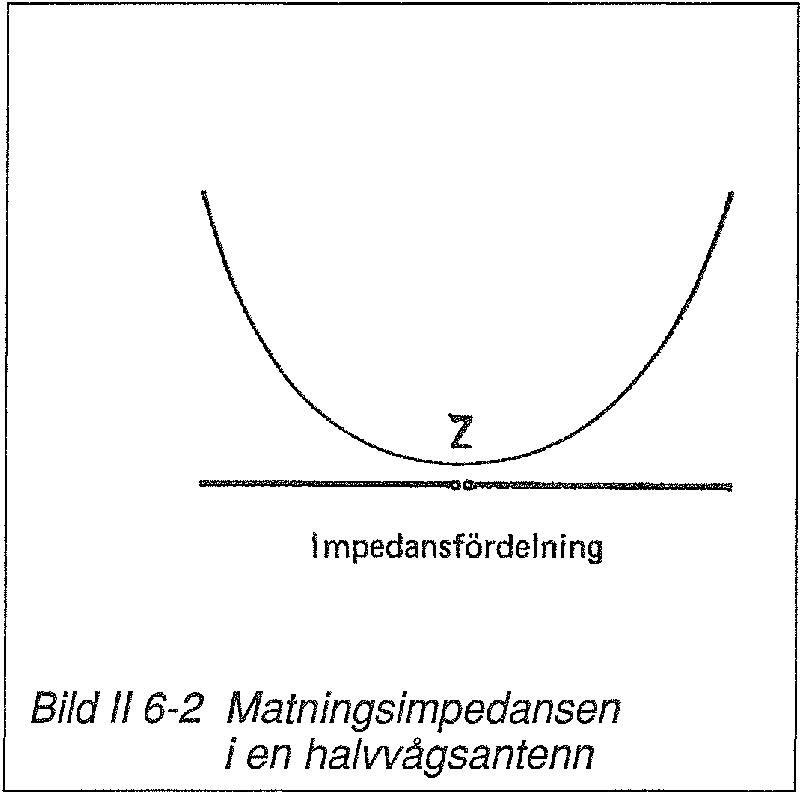
\includegraphics[width=0.5\textwidth]{images/bild_2_6-02.png}
  \caption{Matningsimpedansen i en halvvågsantenn}
  \label{fig:bildII6-2}
\end{wrapfigure}

\begin{figure}
  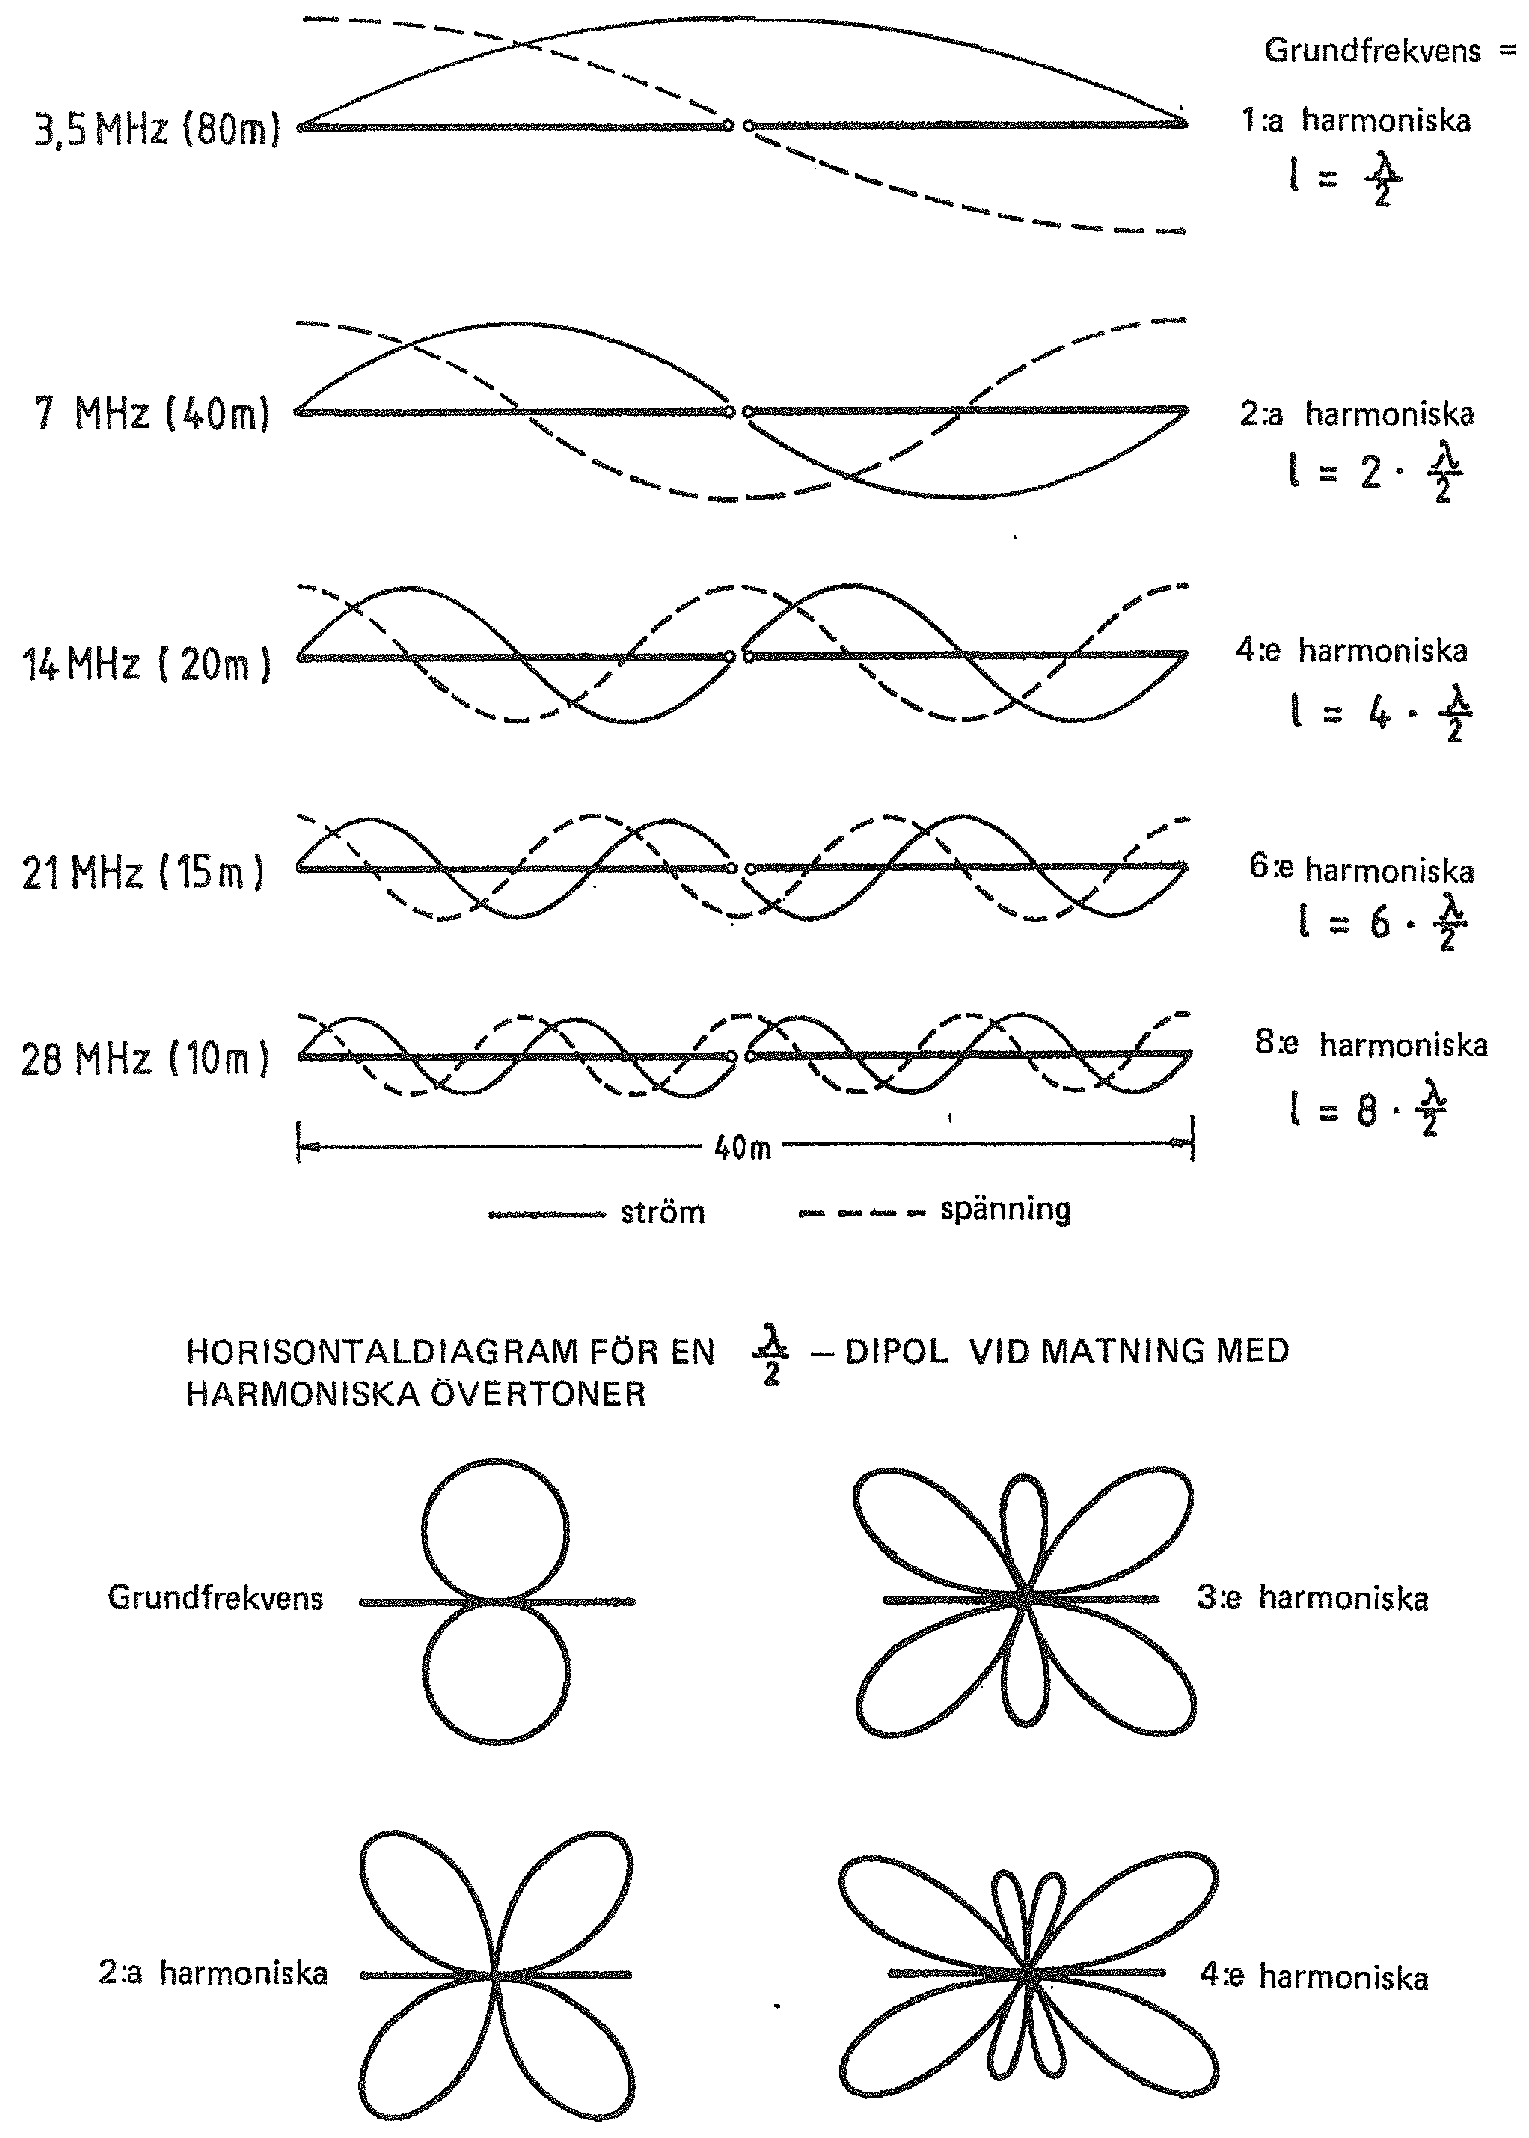
\includegraphics[width=\textwidth]{images/bild_2_6-03.png}
  \caption{Halvvågsdipol matad med harmoniska övertoner}
  \label{fig:bildII6-3}
\end{figure}

Impedansen Z för varje punkt på en antenn kan beräknas med Ohms lag
\(Z = \frac{U}{I}\).

Bild \ref{fig:bildII6-2}

I mitten av en halvvågsantenn på grundfrekvensen är impedansen \(Z\)
låg eftersom spänningen är låg där och strömmen hög. Ute i ändarna är
däremot impedansen hög eftersom spänningen där är hög och strömmen
låg.

Impedansen i mittpunkten är 73~Ω på grundfrekvensen, när antennen mätt
i våglängder befinner sig mycket högt över jordytan, d.v.s. utan
nämnvärd påverkan från omgivningen. I praktiken kan impedansen avvika
mycket från detta värde.

Antenn och matningskabel måste vara impedansanpassade till varandra
för att det inte ska uppstå vågreflexion i anslutningen.

Märk, att halvvågsantennen är i resonans inte bara på grundtonen utan
även på jämna övertoner, 2:a, 4:e etc. harmoniska, varvid
matningspunkten har hög impedans. Vid matning med en lågohmig
koaxialkabel uppstår då en kraftig missanpassning i anslutningen
mellan antenn och kabel, vilket måste åtgärdas på något sätt. Se
avsnitt \ref{transmissionsledningar} i detta kapitel.

\subsubsection{Matningsimpedansen i några antenner}
\index{W3DZZ-antenn}
\index{antenn!W3DZZ}
\index{omvikt dipol}
\index{antenn!omvikt dipol}
\index{folded dipol}
\index{jordplanantenn}
\index{antenn!jordplan}
\index{GP-antenn}
\index{antenn!GP}
\index{yagiantenn}
\index{Yagi-Uda-antenn}
\index{antenn!yagi}
\index{antenn!Yagi-Uda}
\index{Quad-antenn}
\index{antenn!Quad}

Med W3DZZ-antennen (se avsnitt \ref{W3DZZ}) löses hjälpligt anpassningsproblemet med
mittmatade partier på 2:a harmoniska övertonen, d.v.s. dubbla
grundfrekvensen. På 80- och 40~m-banden är antennens matningsimpedans
ca 60~Ω och på de högre banden ca 120~Ω. En kompromiss är att mata
denna antenn med en 75~Ω-kabel för att inte få alltför stor
missanpassning på något band.

\emph{Den omvikta dipolen (folded dipole):}
Matningsimpedansen är ca 240~Ω. En bandkabel med impedansen 300~Ω kan
användas alternativt en koaxialkabel med impedansen 50 eller 75~Ω över
en transformator med impedansomsättningen 4:1.

\emph{Jordplanantennen (GP-antennen):} Matningsimpedansen är 30--60~Ω.
När jordplanets spröt inte riktas horisontellt, utan snett nedåt,
erhålls en matningsimpedans av 50~Ω, vilket passar bra för en
koaxialkabel med 50~Ω impedans.

\emph{Yagi- och Quad-antenner:} En anpassningsanordning för anslutning
av 50--60~Ω koaxialkabel ingår oftast i fabriksgjorda
riktantenner. En 50--60~Ω koaxialkabel kan då användas direkt.

\subsubsection{Reaktansen i en icke-resonant antenn}
\textbf{
HAREC a.\ref{HAREC.a.6.2.3}\label{myHAREC.a.6.2.3}
}
\index{reaktans!antenn}
\index{antenn!reaktans}

Den elektriska svängningskretsen behandlas i avsnitt \ref{oscillatorer}. Där framställs
svängningskretsens grundegenskaper resistans \(R\), induktans \(L\)
och kapacitans \(C\) som koncentrerade till komponenter kallade
resistor, induktor respektive kondensator.

Även en enkel tråd har dessa egenskaper, men utfördelade över hela
tråden. Denna kan därför ses som ett stort antal komponenter, som
tillsammans bildar en svängningskrets, vilken naturligtvis kan fungera
som antenn.

När antennen matas med växelström med samma frekvens som antennens
resonansfrekvens, så svänger antennen med de minsta
förlusterna. Resonansfallet kan i korthet beskrivas så att den
induktiva och kapacitiva reaktansen i antennen tar ut varandra medan
resistansen kvarstår.

Impedansen är vektorsumman av resistansen och de kapacitiva och
induktiva reaktanserna. I resonans är antennens impedans lika med
resistansen, vilket är ett specialfall. Antennströmmen har alltid
sändarens frekvens. Om sändningsfrekvensen är en annan än antennens
resonansfrekvens, så händer endera av följande: När antennströmmen har
lägre frekvens än antennens resonansfrekvens, så blir den resulterande
reaktansen negativ (kapacitiv), d.v.s. \(X_C\) är större än \(X_L\).

När antennströmmen har högre frekvens än antennens resonansfrekvens,
så blir den resulterande reaktansen positiv (induktiv), d.v.s. \(X_L\)
är större än \(X_C\).

\subsection{Elektrisk ''förlängning'' och ''förkortning''}
\index{elektrisk förlängning}
\index{antenn!elektrisk förlängning}
\index{elektrisk förkortning}
\index{antenn!elektrisk förkortning}

\begin{wrapfigure}{R}{0.5\textwidth}
  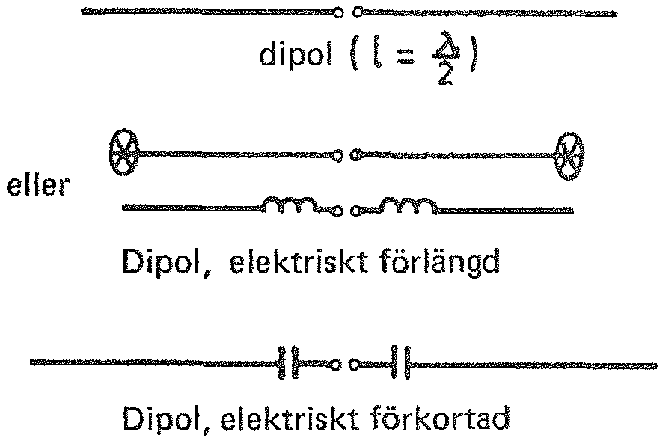
\includegraphics[width=0.5\textwidth]{images/bild_2_6-04.png}
  \caption{Elektrisk förlängning och förkorting av antenner}
  \label{fig:bildII6-4}
\end{wrapfigure}

Om sändarfrekvensen, avviker mycket från antennens resonansfrekvens,
så kan reaktansen i antennen behöva elimineras eller åtminstone
minskas för en bättre impedansanpassning mellan antenn och
matarledning. Den enklaste åtgärden är då att försöka ändra
antennlängden.

Bild \ref{fig:bildII6-4}

Om detta inte låter sig göras, så kan man i serie med en ''för kort''
antenn sätta in en induktor -- en s.k. elektrisk förlängning. Om i
motsatt fall antennen är ''för lång'', så kan man sätta in en
kondensator en s.k. elektrisk förkortning.

I amatörradio ändras sändarfrekvensen mycket och ofta, varför
antennsystemet bör kunna stämmas av från marken/operatörsplatsen. Då
kan en antennkopplare med nödvändiga reaktiva komponenter behövas.  Se
längre fram i kapitlet.

\subsection{Anpassning till sändarens impedans}
\textbf{
HAREC a.\ref{HAREC.a.5.3.7}\label{myHAREC.a.5.3.7}
}
\index{avstämningsanordning}
\index{match}
\index{sändare!match}
\index{impedansanpassning}
\index{sändare!impedansanpassning}
\index{π-filter}
\index{sändare!π-filter}
\index{ståendevåg}

Ett sändarslutsteg med elektronrör är vanligen utrustat med en
\emph{avstämningsanordning} (eng. \emph{matching network} och \emph{match})
vid HF-utgången. Syftet är att kunna anpassa
sändarens utgångsimpedans till impedansen i antennledningen. I moderna
sändare består denna anordning mycket ofta av ett s.k. π-filter, vars
utgångsimpedans kan variera mellan ca 30--150~Ω.

Ett transistoriserat slutsteg är oftast utfört för en fast
utgångsimpedans av 50~Ω och är alltså i behov av en
avstämningsanordning, om inte antennsystemet inom vissa gränser håller
samma impedans. Toleransgränsen för felanpassning brukar vara ett SVF
av storleksordningen 2:1 innan sändarens skyddskretsar styr ner
uteffekten.

Vid lika impedans i sändarutgång, matarledning och antennanslutning
uppträder ingen stående våg på matarledningen och mesta möjliga effekt
överförs från sändaren till antennen.

\subsection{Antennens strålningsdiagram}
\index{strålningsdiagram}
\index{antenn!strålningdiagram}

\begin{figure}
  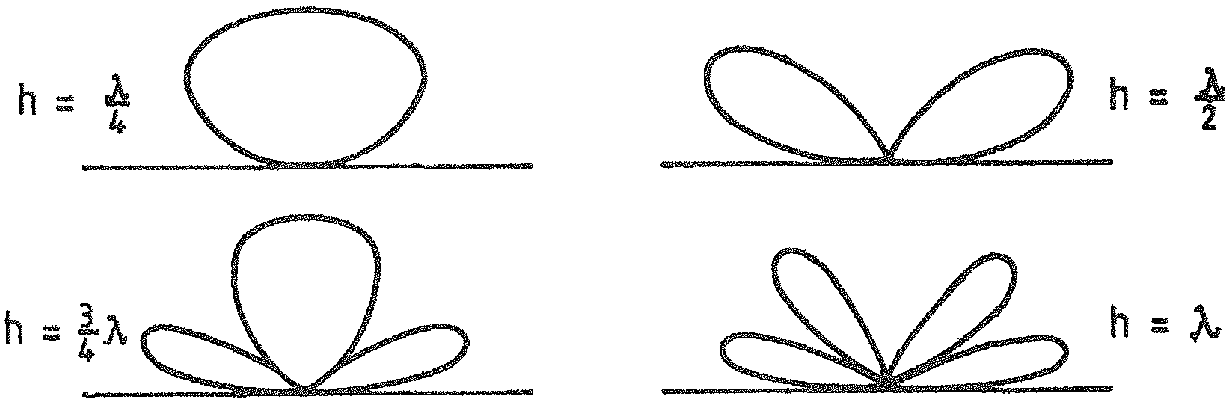
\includegraphics[width=\textwidth]{images/bild_2_6-05.png}
  \caption{Vertikaldiagram för halvvågsantenn}
  \label{fig:bildII6-5}
\end{figure}

En antenns strålningsbild beskrivs bäst i tre dimensioner. Bild \ref{fig:bildII6-3}
visar bl.a. ett horisontaldiagram för en halvvågsantenn.

Bild \ref{fig:bildII6-5} visar strålningen i vertikalplanet som funktion av
antennhöjden för samma antenn. Vertikaldiagrammet kan ha mycket olika
utseende beroende på antennens utförande, dess elektriska höjd över
mark och omgivningens elektriska egenskaper. För att överbrygga stora
avstånd, måste antennen ha en flack utstrålning relativt
markplanet. En horisontelit upphängd antenn med en längd av
\(\lambda/2\) har övervägande flack utstrålning när den placeras på en
höjd av \(\lambda/2\), \(\lambda\), \(3\lambda/2\), \(2\lambda\),
o.s.v. över mark. När en horisontell antenn däremot placeras
\(\lambda/4\), \(3\lambda/4\), \(5\lambda/4\) o.s.v. över mark, är
utstrålningen övervägande vertikal, vilket inte ska förväxlas med
polarisationen, som i detta fall är horisontell.

Samma diagram gäller både för en sändar- och mottagarantenn. styrkan
på en utstrålad signal motsvaras av styrkan på mottagen signal.

\subsection{Antennvinst}
\textbf{
  HAREC a.\ref{HAREC.a.6.2.5}\label{myHAREC.a.6.2.5}
}
\index{antennvinst}
\index{antenn!antennvinst}
\index{isotropisk antenn}
\index{antenn!isotropisk}
\index{symbol!G antennvinst}
\index{dBi isotropiskt gain}
\index{antenn!dBi isotropiskt gain}
\index{isotropiskt gain (dBi)}
\index{antenn!isotropiskt gain (dBi)}
\index{dBd dipol gain}
\index{antenn!dBd dipol gain}
\index{dipol gain (dBd)}
\index{antenn!dipol gain (dBd)}

Med \emph{antennvinst} \(G\) (eng. \emph{antenna gain}) menas förhållandet
mellan effekten \(P_t\) i huvudstrålningsriktningen (framriktningen för en
antenn med osymmetriskt utstrålad effekt) och effekten från en definierad
referensantenn.

Förmågan att ha högre antennvinst i en riktning i förhållande till andra
riktningar kallas för direktivitet (eng. \emph{antenna directivity}).

En referensantenn som tänks vara oändligt liten och som strålar med exakt
samma effekt \(P_t\) i alla riktningar kallas \emph{isotropisk antenn}.
En isotropisk antenn är emellertid endast teoretisk definierbar.

Med effekten \(P_i\) från den isotropiska antennen som referens blir
antennvinsten

\[G = 10 \log\frac{P_t}{P_i} \quad \text{[dBi]}\]

En i praktiken definierbar referens är halvvågsdipolen, vars
huvudstrålning är vinkelrätt ut från dipolen och runt omkring den.
Referenseffekten är då \(P_d\) och antennvinsten

\[G = 10 \log\frac{P_t}{P_d} \quad \text{[dBd] Bild \ref{fig:bildII6-6}}\]

Bild \ref{fig:bildII6-6}

\begin{wrapfigure}{R}{0.5\textwidth}
  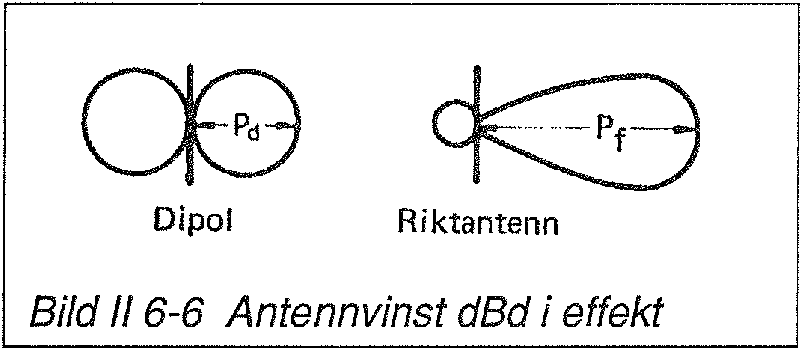
\includegraphics[width=0.5\textwidth]{images/bild_2_6-06.png}
  \caption{Antennvinst dBd i effekt}
  \label{fig:bildII6-6}

  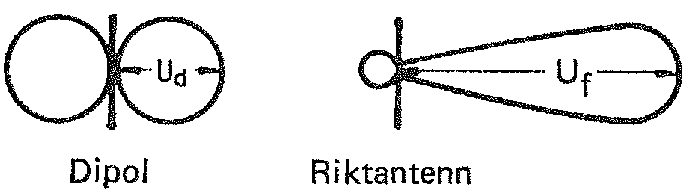
\includegraphics[width=0.5\textwidth]{images/bild_2_6-07.png}
  \caption{Antennvinst dBd i spänning}
  \label{fig:bildII6-7}
\end{wrapfigure}

Antennvinsten kan också definieras som förhållandet mellan den
elektriska fältstyrkan uf i huvudstrålningsriktningen och
referensfältstyrkan (dipol).

Jämfört med \(\lambda/2\)-dipol är antennvinsten

\[G = 20 \log\frac{U_t}{U_d} \quad \text{[dBd] Bild \ref{fig:bildII6-7}}\]

Man använder uttrycket dBi när antennvinsten anges i förhållande till
en isotrop antenn och dBd i förhållande till en halvvågsantenn.  Se
appendix \ref{decibel} om decibelbegreppet.

Exempel på beräkning av antennvinst:

\begin{align*}
  U_f &= 40\text{ µV} \quad U_d = 20\text{ µV} \quad G =\ ? \\
  G &= 20 \log\frac{U_f}{U_d} = 20 \log\frac{40}{20} \\
  &= 20 \log 2 = 20\cdot 0.3 = 6 \quad \text{[dBd]} \\
\end{align*}

6~dB antennvinst motsvarar en fördubblad fältstyrka [V/m], d.v.s. 1~S-enhets
ökning vid den mottagande stationen, liksom att 6~dB antennvinst motsvarar
en 4-faldigad sändareffekt \(\mathrm{[W/m^2]}\).

Ungefärlig antennvinst för olika antenner med en isotropantenn som referens:
\begin{tabular}{l|ll|ll}
  & \multicolumn{2}{l|}{\(\lambda/2\)-dipol} &
  \multicolumn{2}{l}{Isotrop} \\
  \hline
  Isotrop antenn       & -2,1 & dBd & 0   & dBi \\
  GP, \(\lambda/4\)    & -1,8 & dBd & 0,3 & dBi \\
  Dipol, \(\lambda/2\) & 0    & dBd & 2,1 & dBi \\
  GP, \(5/8\lambda\)   & 1,2  & dBd & 3,3 & dBi \\
  & & & & \\
  Dipol, \(1/1\lambda\) & 1,8 & dBd & 3,9  & dBi \\
  2-elements yagi       & 5   & dBd & 7,1  & dBi \\
  2-elements quad       & 6   & dBd & 8    & dBi \\
  3-elements yagi       & 8   & dBd & 10,1 & dBi \\
\end{tabular}

Antennen har egna förluster, det gör att olika antenner kan ha olika
effektivitet, därför finns måttet antenneffektivitet
(eng. \emph{antenna efficiency}) \(\eta\) som beror på relationen mellan
utstrålningsresistansen \(R_R\) och förlustresistansen \(R_L\)

\[\eta = \frac{R_R}{R_R+R_L}\]

\subsection{Effektivt utstrålad effekt}
\textbf{
HAREC a.\ref{HAREC.a.6.2.7}\label{myHAREC.a.6.2.7}
}
\index{effektivt utstrålad effekt (ERP)}
\index{antenn!effektivt utstrålad effekt (ERP)}
\index{ERP Effective Radiated Power}
\index{antenn!ERP Effective Radiated Power}
\index{ekvivalent isotropiskt utstrålad effekt (EIRP)}
\index{antenn!ekvivalent isotropiskt utstrålad effekt (EIRP)}
\index{EIRP Equivalent Isotropically Radiated Power}
\index{antenn!EIRP Equivalent Isotropically Radiated Power}

Effektivt utstrålad effekt (ERP) (eng. \emph{effective radiated power}) är den
effekt som sändarantennen strålar ut i sin bästa
strålningriktning. ERP beräknas som den effekt som tillförs själva
antennen, multiplicerat med antennvinsten relativt en
halvvågsdipol. Förlusterna på vägen från sändaren ut till antennen är
alltså borträknad före beräkningen av ERP.

Ekvivalent isotropiskt utstrålad effekt (EIRP) (eng. \emph{Equivalent isotropically radiated power}).
EIRP beräknas relativt en teoretisk antenn (\emph{isotropisk antenn}) som 
strålar lika mycket i alla riktningar. Vid beräkningen används den effekt
som tillförs själva antennen, multiplicerat med antennvinsten relativt en
isotrop. Förlusterna på vägen från sändaren ut till antennen är liksom vid beräkningen av ERP borträknade vid beräkningen av EIRP.

\subsection{Fram-/backförhållande (antennvinst)}
\textbf{
HAREC a.\ref{HAREC.a.6.2.8}\label{myHAREC.a.6.2.8}
}
\index{fram/backförhållande}
\index{antenn!fram/backförhållande}

Med fram-/backförhållande (F/B) för en riktantenn menas förhållandet
mellan den utstrålade effekten i framriktningen \(P_f\) och effekten i
backriktningen \(P_b\).

\[ F/B = 10 \log\frac{P_f}{P_b} \quad \text{[dB]} \]

\begin{wrapfigure}{R}{0.5\textwidth}
  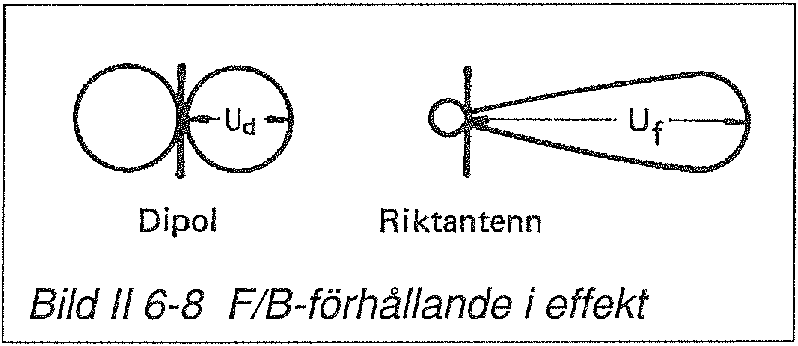
\includegraphics[width=0.5\textwidth]{images/bild_2_6-08.png}
  \caption{F/B-förhållande i effekt}
  \label{fig:bildII6-8}
\end{wrapfigure}

Fram/backförhållandet kan också definieras som förhållandet mellan
elektriska fältstyrkan \(U_f\) i framriktningen och
referensfältstyrkan \(U_b\) i backriktningen

\[ F/B = 20 \log\frac{U_f}{U_b} \quad \text{[dB]} \]

\begin{wrapfigure}{R}{0.5\textwidth}
  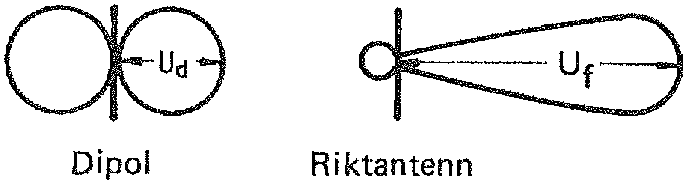
\includegraphics[width=0.5\textwidth]{images/bild_2_6-09.png}
  \caption{F/B-förhållande i spänning}
  \label{fig:bildII6-9}
\end{wrapfigure}

Exempel 1:

\begin{align*}
  U_f &= 40 \text{ µV} \quad U_b = 4\text{ µV} \quad F/B =\ ? \\
  F/B &= 20 \log\frac{U_f}{U_b} = 20 \log{40}{4} \\
  &= 20 \log 10 = 20 \cdot 1 = 20 \quad \text{[dB]} \\
\end{align*}

\(F/B = 20\) dB betyder att fältstyrkan \(U_f\) i huvudriktningen är
10 gånger så hög som referensfältstyrkan \(U_b\).

Exempel 2:

\begin{align*}
  U_f &= 15 \text{ µV} \quad U_b = 15\text{ µV} \quad F/B =\ ? \\
  F/B &= 20 \log\frac{U_f}{U_b} = 20 \log\frac{15}{15} \\
  &= 20 \log 1 = 20 \cdot 0 = 0 \quad \text{[dB]} \\
\end{align*}

\(F/B = 0\) dB betyder att \(U_t = U_b\), d.v.s. att fältstyrkorna i
fram- och backriktning är lika stora, vilket inträffar för en dipol.

\subsection{Halvvärdesbredd}
\index{halvvärdesbredd}
\index{antenn!halvvärdesbredd}

Studera diagrammet för den horisontella strålningen från en riktantenn.

Antennen avger sin största utstrålade effekt \(P_f\) i
huvudriktningen. Effekten avtar utanför huvudriktningen. Fältstyrkan
Ut förhåller sig på liknande sätt.

Med effekthalvvärdesbredd menas den vinkel inom vilken nyttoeffekten
är minst hälften så stor som i huvudriktningen.

Bild \ref{fig:bildII6-10}

\begin{gather*}
  \text{Observera, att } \frac{P_f}{2} \text{ motsvarar }
  \sqrt{\frac{1}{2}}U_f \\
  ( \approx 0,7 U_f \text{ motsvarande 3 dB })
\end{gather*}

Med spänningshalvvärdesbredd menas den vinkel inom vilken spänningen
(fältstyrkan) är minst hälften så stor som den största nyttospänningen
\(U_f\). Spänningshalvvärdesbredden på en dipol är ungefär 90°.

\begin{figure}
  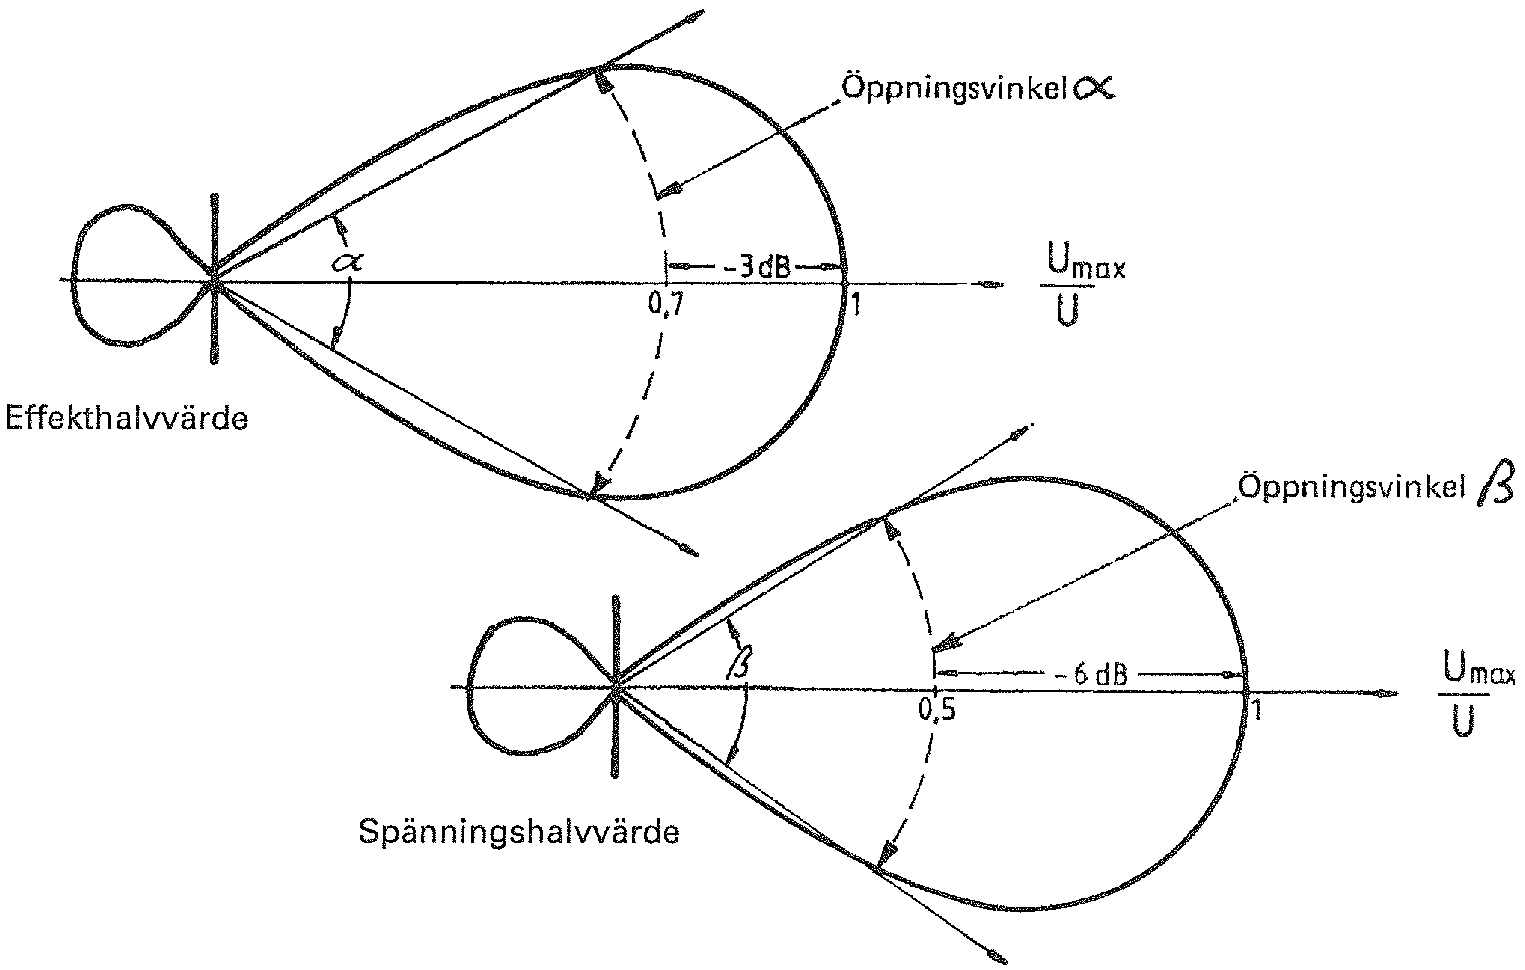
\includegraphics[width=\textwidth]{images/bild_2_6-10.png}
  \caption{Halvvärdesbredder}
  \label{fig:bildII6-10}
\end{figure}
